\documentclass[a4paper, amsfonts, amssymb, amsmath, reprint, showkeys, nofootinbib, twoside]{revtex4-1}
\usepackage[english]{babel}
\usepackage[utf8]{inputenc}
\usepackage[colorinlistoftodos, color=green!40, prependcaption]{todonotes}
\usepackage[pdftex, pdftitle={Article}, pdfauthor={Author}]{hyperref}
\usepackage{amsthm}
\usepackage{mathtools}
\usepackage{physics}
\usepackage{xcolor}
\usepackage{caption}
\usepackage{hyperref}
%\hypersetup{colorlinks=true, linkcolor=blue, urlcolor = blue}
\usepackage{amsmath}
\usepackage{amssymb}
\usepackage{graphicx}
\graphicspath{Images}
\usepackage[left=23mm,right=13mm,top=35mm,columnsep=15pt]{geometry} 
\usepackage{adjustbox}
\usepackage{placeins}
\usepackage[T1]{fontenc}
\usepackage{float}
%\usepackage{longtable}
\usepackage{csquotes}
\usepackage{refstyle}
\usepackage{lipsum}
\usepackage{booktabs}



\begin{document}

\title{Determination of wavelength of light using Fabry-Pérot Interferometer}
\author{Swaroop Ramakant Avarsekar}
\email{swaroop.avarsekar@niser.ac.in}
\affiliation{School of Physical Sciences, National Institute of Science Education and Research, HBNI, Jatni -752050, India}
\date{\today}


	
\begin{abstract}
Fabry-Pérot Interferometer is based on the principle of multiple beam interference, where multiple reflections takes place between the etalon giving rise to concentric fringes. The sharpness of these fringes depends on coefficient of Finesse, which depends on the net reflectivity. From the Fabry-Pérot interferometer we can determine the wavelength of light used (LASER) and distance between etalon. We obtained wavelength of laser $\lambda$ as $766.26\pm1.69$ nm and distance between etalon (d) as $2.90\pm 0.14$ mm.
\end{abstract}
	
\keywords{Interferometer, Etalon, Coefficient of Finesse,}
	
\maketitle

\section{Introduction}
Fabry-Pérot Interferometer is based on the principle of multiple beam interferometry. The light passes through two reflective parallel glass plates, known as Fabry-Pérot etalon, where some portion of light is transmitted as well as reflected, these multiple beams interfere with each other. The intensity of interference maxima is higher as number of reflections is more. If additional optical path length of reflected beam is a integral multiple of wavelength of light, it results in constructive interference.

\section{Theory}
\begin{figure}[htbp] %  figure placement: here, top, bottom, or page
   \centering
   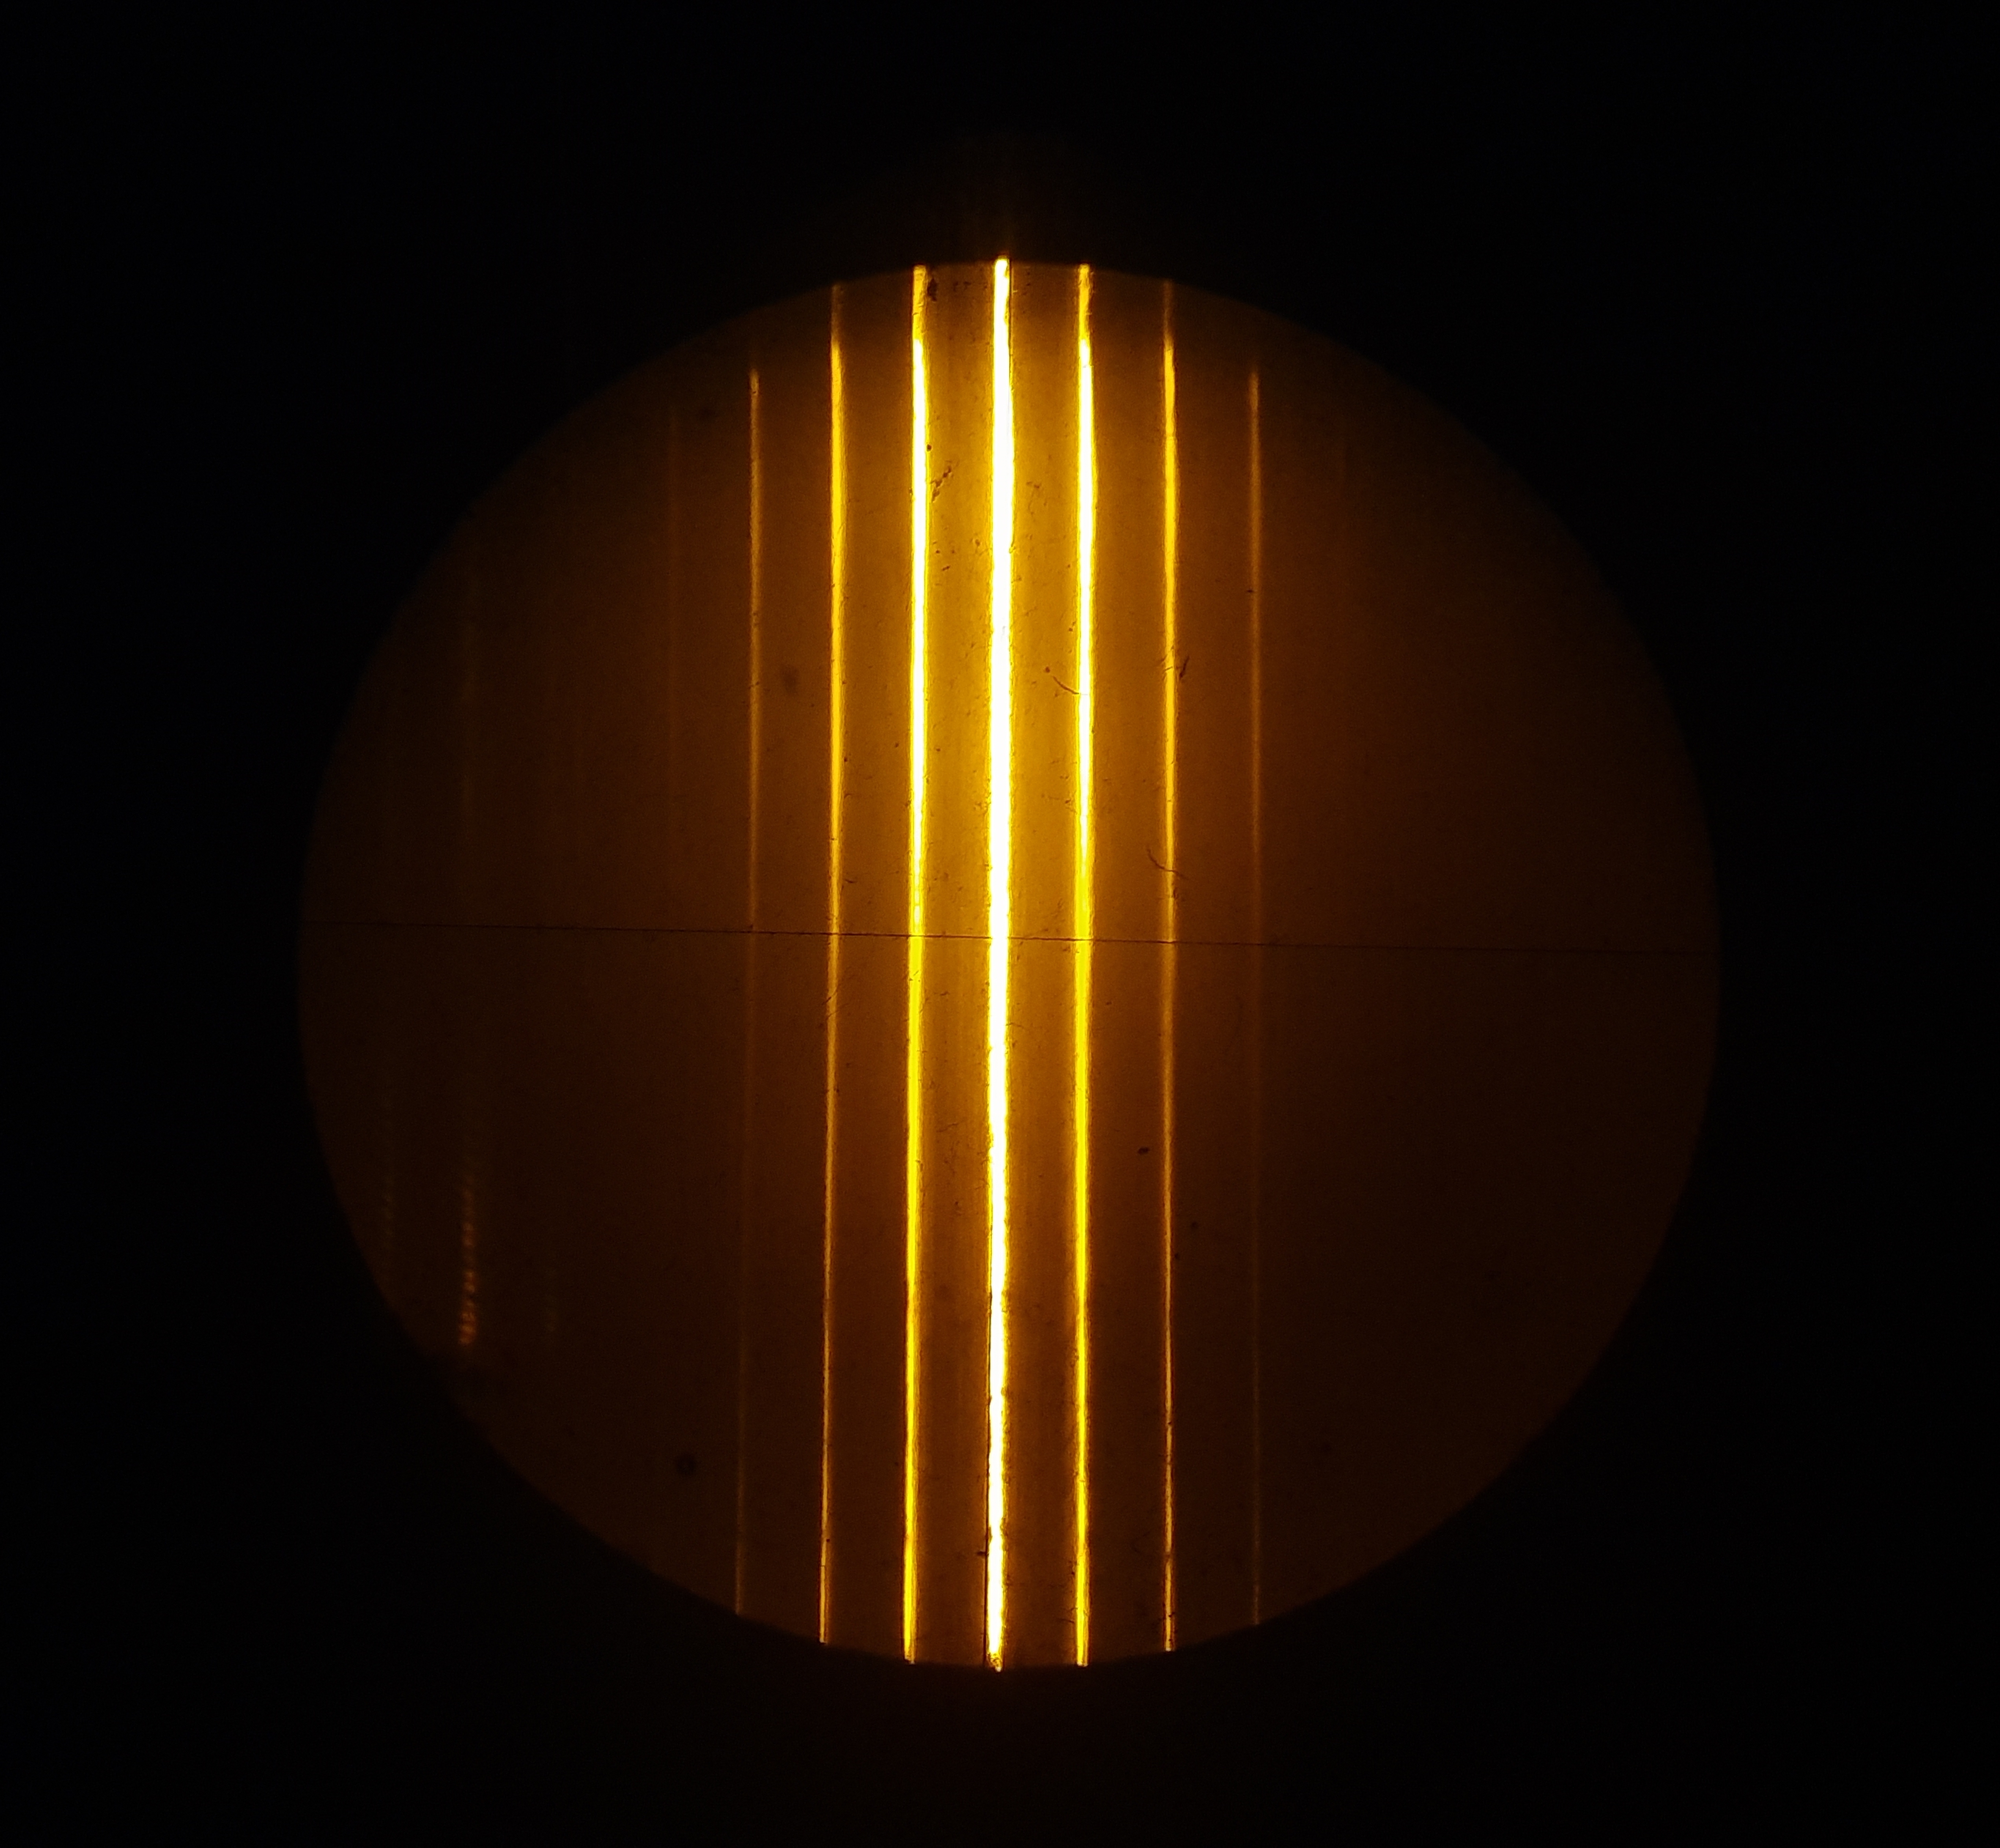
\includegraphics[width=3in]{1} 
   \caption{Reflection and transmission of a beam incident at an angle $\theta$ on a film.}
   \label{1}
\end{figure}

If $A_o$ is the amplitude of the incident wave, it undergoes multiple reflections at the two interfaces. Let $r_1$ \& $t_1$ be the reflecting and transmitting coefficients when the light travels from $n_1$ to $n_2$, respectively. Also, $r_2$ \& $t_2$ be the corresponding coefficients for light travelling from  $n_2$ to $n_1$, respectively. The amplitude of successive reflected waves would be $A_0 r_1$, $A_o t_1 r_2 t_2 e^{i\delta}$ , $ A_o t_1 r_2^{3}  e^{2i\delta}$...where,

\begin{equation}
\delta=\frac{2\pi\Delta}{\lambda_o}= \frac{4\pi n_2 h cos\theta_2}{\lambda_o}
\end{equation}
\newline
$\delta$ represents phase difference between two waves emanating from plates due to additional path traversed by the beam in the film. We also know that $r_1$=$-r_2$, $|r_1|^2+t_1t_2=|r_2|^2+t_1t_2=1$, $R=|r_1|^2=|r_2|^2$ and $T=t_1t_2=1-R$

Therefore, the resultant amplitude of the reflected wave is 
\begin{equation}
A_r=A_o[r_1+t_1t_2r_2 e^{i\delta}(1+r_2^{2}e^{i\delta}+r_2^{4}e^{2i\delta}+...)]
\end{equation}

Therefore,
\begin{equation}
A_r=A_o\left[r_1+\frac{t_1t_2r_2 e^{i\delta}}{1-r_2^{2}e^{i\delta}}\right]
\end{equation}

So, from the above equations,
\begin{equation}
\frac{A_r}{A_o}=r_1\left[1-\frac{(1-R) e^{i\delta}}{1-Re^{i\delta}}\right]=r_1\frac{(1-e^{i\delta})}{(1-Re^{i\delta})}
\end{equation}

Net reflectivity is calculated by 
\begin{equation}
\mathcal{R}=\left|\frac{A_r}{A_o}\right|^2=R\left|\frac{1-e^{i\delta}}{1-Re^{i\delta}}\right|^2
\end{equation}

\begin{equation}
\mathcal{R}=\frac{4Rsin^{2}(\frac{\delta}{2})}{(1-R)^2+4Rsin^{2}(\frac{\delta}{2})}
\end{equation}

\begin{equation}
\mathcal{R}=\frac{Fsin^{2}(\frac{\delta}{2})}{1+Fsin^{2}(\frac{\delta}{2})}
\end{equation}

where $F=\frac{4R}{(1-R)^2}$ is called coefficient of Finesse.

The resultant transmission is given by, 
\begin{equation}
\mathcal{T}=1-\mathcal{R}=\frac{1}{1+Fsin^{2}(\frac{\delta}{2})}
\end{equation}

\begin{figure}[htbp] %  figure placement: here, top, bottom, or page
   \centering
   \includegraphics[width=3.3in, height=1.8in]{sc} 
   \caption{Schematic diagram of Fabry-Pérot Interferometer}
   \label{2}
\end{figure}

\begin{figure}[htbp] %  figure placement: here, top, bottom, or page
   \centering
   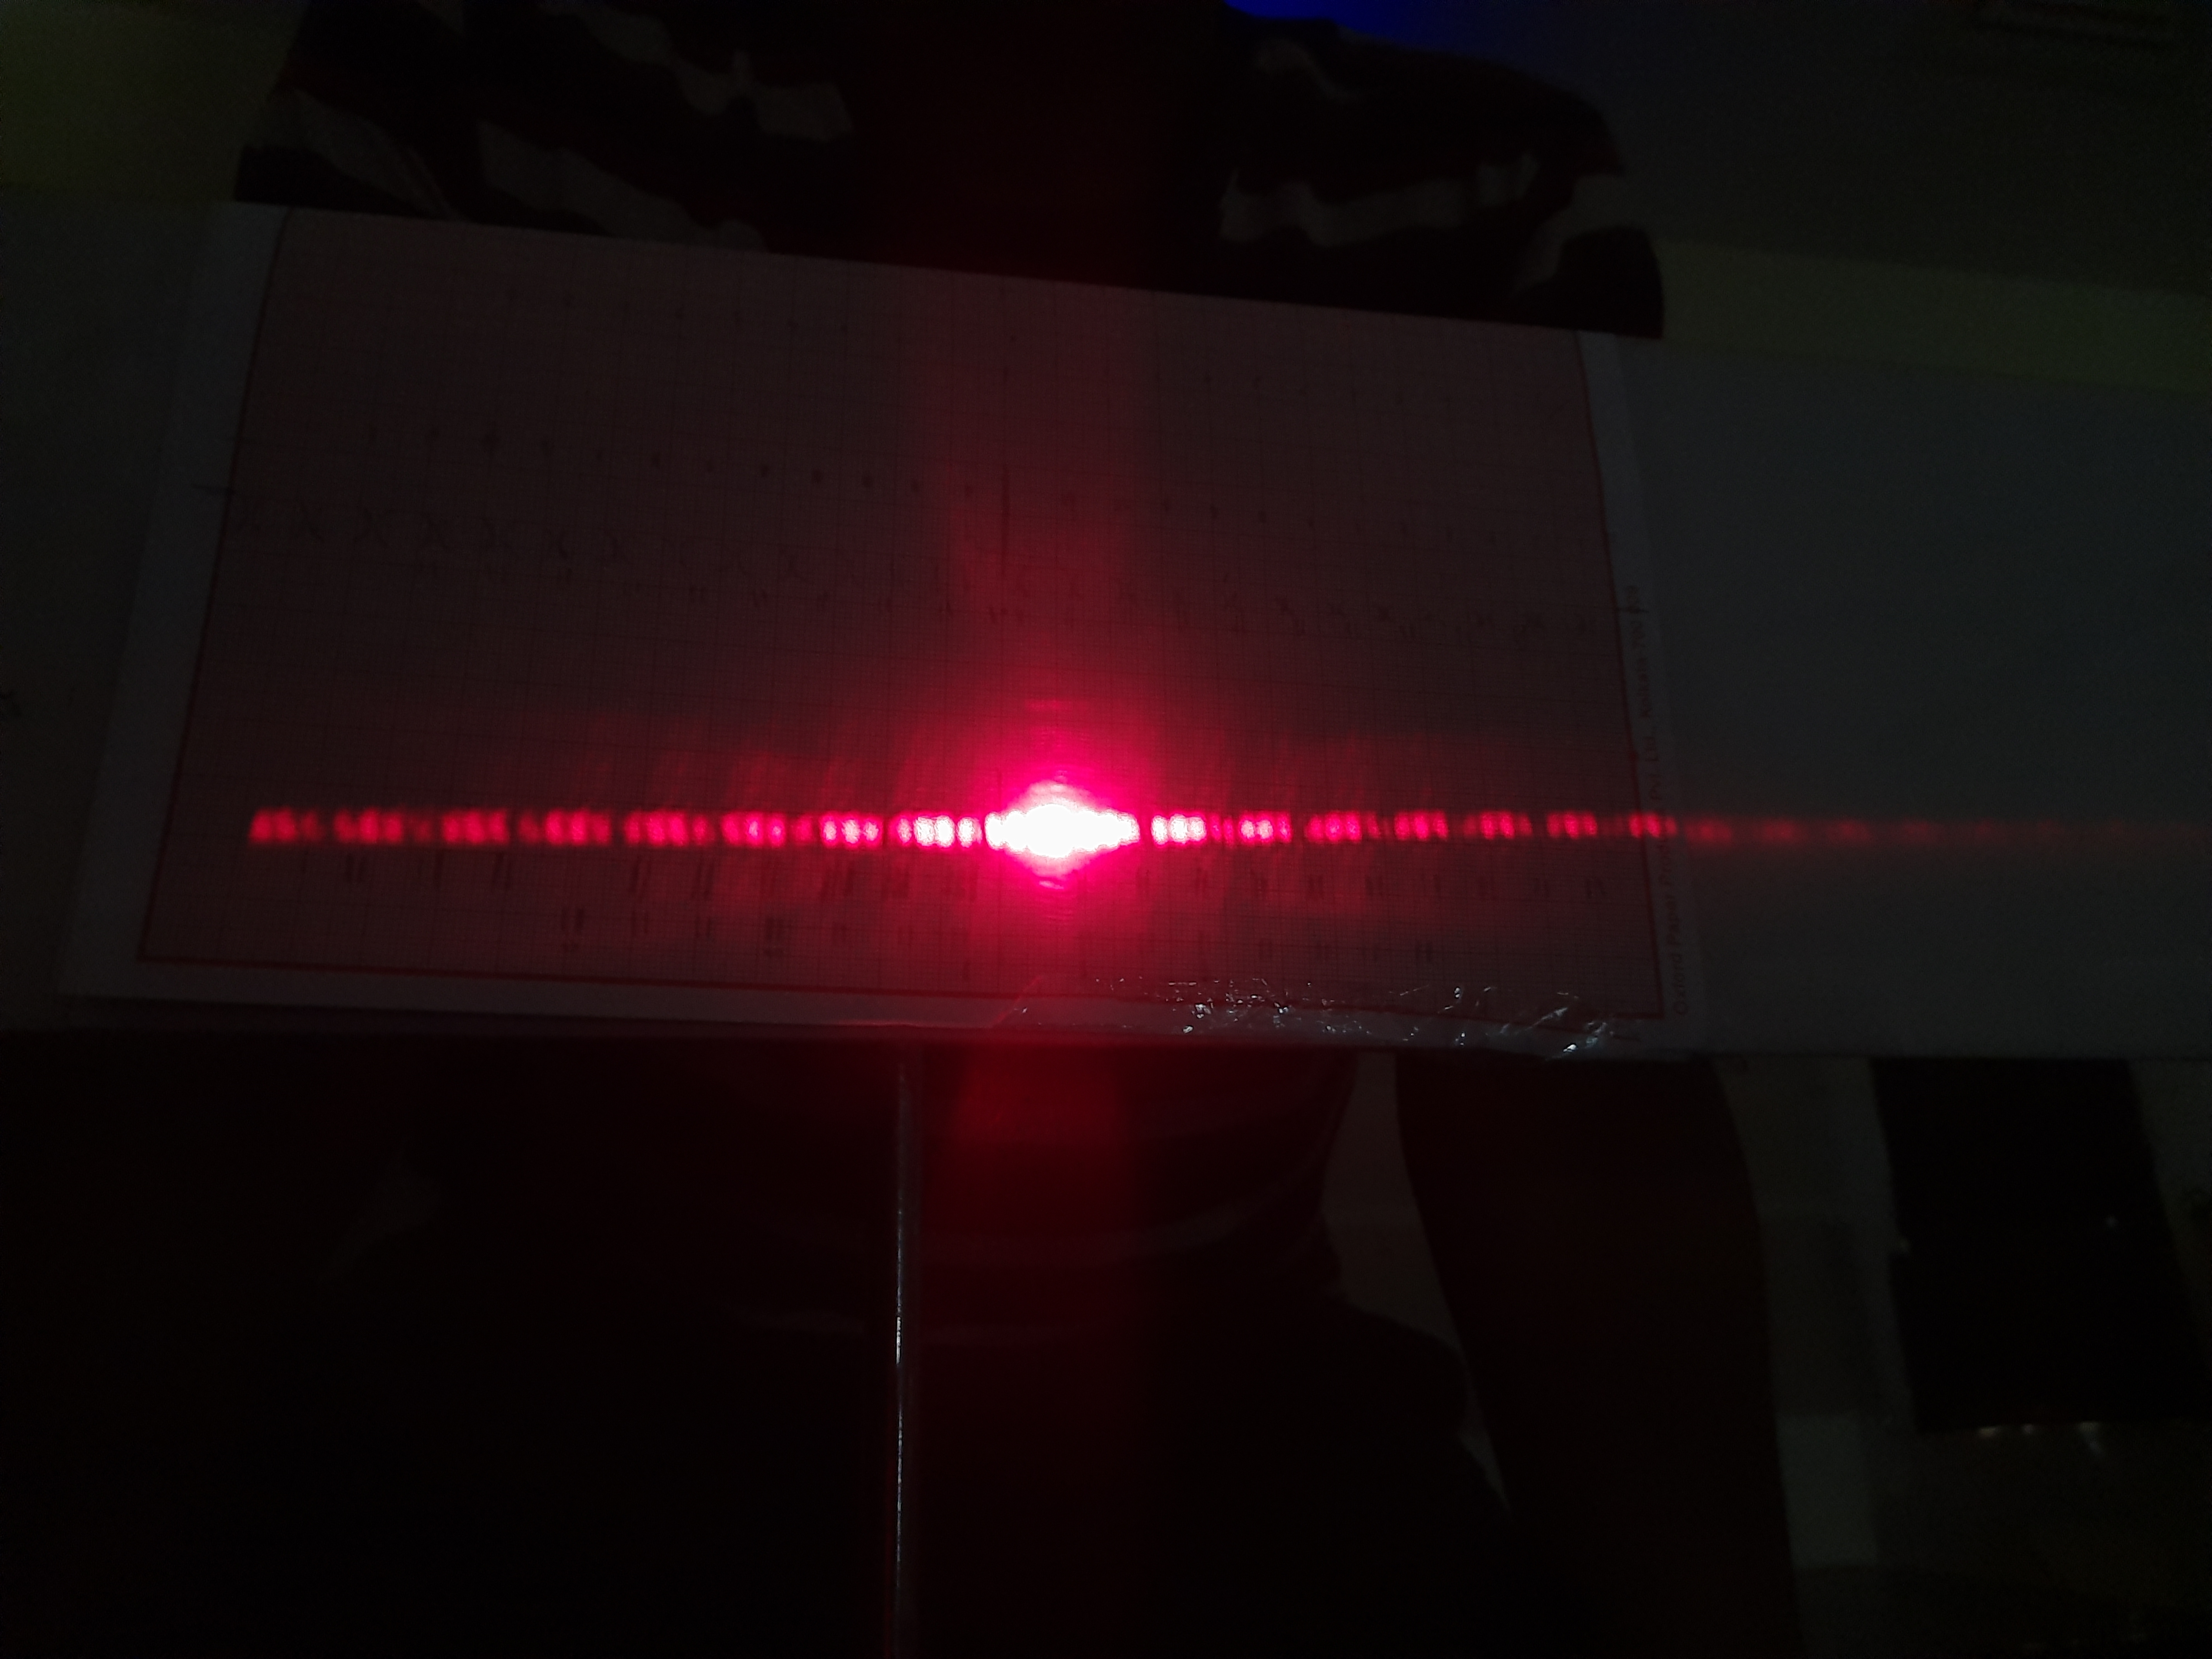
\includegraphics[width=3.3in, height=1.8in]{4} 
   \caption{Finesse is the measure of the sharpness of transmission peaks for $\mathcal{T}=1$.}
   \label{2}
\end{figure}

If $I_o$ is the incident intensity, and $I_t$ is transmitted light intensity, then $I_t$ is maximum if $\delta=2m\pi$ , $\Delta=m\lambda$ and minima for $\delta=(2m+1)\pi$, $\Delta=(2m+1)\lambda$ for m=0, 1, 2, 3...The interference pattern appears as concentric fringes where sharpness will depend on coefficient of Finesse, $F$. The optical path difference between two consecutive light beam is 
\begin{equation}
\Delta=2ndcos\theta
\end{equation}

where n is the refractive index of medium in cavity.

To determine the wavelength of the light used, the medium in the etalon is air ($n\approx1$), with the separation as $d_1$ initially. If we count the number of fringes appearing/collapsing at the centre, where $\theta\approx0$, by varying the separation to $d_2$ then,
\newline
$$2d_1=m_1\lambda$$  $$2d_2=m_2\lambda$$
\newline
Therefore by subtracting above equations we get, 
\begin{equation}\label{e1}
\text{Wavelength of light}, \lambda=2\left(\frac{d_1-d_2}{m_1-m_2}\right)
\end{equation}

And to determine the distance between etalon (d), if the radius of $m^{th}$ order fringe is $r_m$ and angle subtended at any point on the circular fringe on the screen kept at a distance $D$, is $\theta_m$. From small angle approximation, $\theta_m=r_m/D$. Therefore, 
\begin{equation}\label{e2}
d=\frac{m\lambda}{2cos\theta_m}
\end{equation}

\section{Experiment}
\subsection{Apparatus}
The experimental apparatus consists of optical rail with carrier, mounting support and optical post with holder for the etalon. One of the mirror mount is movable while other is fixed. A diffusing screen with linear translation stage is also joined to the rail. The pointer on the screen helps to measure the diameter of the fringes. A collimating lens of focal length 10 cm is mounted to focus the laser beam from the laser diode at the other end of the rail. The whole setup can be placed on optical breadboard in order to provide the stability.

\begin{figure}[htbp] %  figure placement: here, top, bottom, or page
   \centering
   \includegraphics[width=3.3in]{3} 
   \caption{Fabry-Pérot Interferometer setup at laboratory}
   \label{setup}
\end{figure}

\subsection{Procedure}
Mount the rail on optical breadboard along with the screen on one end and laser diode in the other end. At the middle of rail, mount the etalon such that there are parallel with each other. Adjust the distance to about 2 mm using micrometer. Align the laser beam such that it passes through the centre of the etalon and hits screen. Place the collimating lens along the same axis , to expand the beam and to observe the concentric interference fringes on the screen. Calculate the least count of the micrometer.

To determine the wavelength of the laser beam, take the initial reading of the micrometer attached to mirror. Let it be $d_1$. Turn the micrometer knob extremely slowly and count number of fringes appearing/ collapsing. Record the micrometer reading as $d_2$ after every set of fringe count. Use equation (\ref{e1}) and plot the graph between $d_1-d_2$ and $m_1-m_2$ to find wavelength of the laser, $\lambda$.

To determine the distance between the etalon plates $d$, measure the distance $D$ between etalon and and the screen. Note the reading of first dark fringe ($a$) on the left side with the pointer, from the scale on the screen. Repeat for consecutive fringes translating along the same direction take the reading on the right side ($b$) as well. The difference $|a-b|$ gives the diameter of the fringes of order m. Calculate the $\theta_m$ and use equation (\ref{e2}) to plot the appropriate graph and calculate $d$.

\subsection{Precautions}
\begin{enumerate}
\item{Conduct the experiment in quiet place free from mechanical disturbances.}
\item{Never make direct eye contact with the laser beam}
\item{Make sure two mirrors never touch each other, doing so may result in damage of the surface.}
\item{Move the micrometer extremely slowly to get the proper count of the fringes as the setup is very sensitive.}
\item{Avoid touching optical surfaces as it may damage the surface coatings.}
\end{enumerate}

\subsection{Observations and Tabular Column}
 Least count of micrometer =0.001 cm

\begin{table}[htbp]
\centering
\caption{To calculate wavelength of light ($\lambda$)}
\label{t2}
Initial position of micrometer, $d_1=2.206$ cm
\begin{tabular}{@{}cccc@{}}
\toprule
Sl.No &
  \begin{tabular}[c]{@{}c@{}}No. of fringes appeared/\\ collapsed ($m_1-m_2$)\end{tabular} &
  \begin{tabular}[c]{@{}c@{}}$d_2$ \\ (cm)\end{tabular} &
  \begin{tabular}[c]{@{}c@{}}$d_1-d_2$ \\ (cm)\end{tabular} \\ \midrule
1 & 52  & 2.204 & 0.002 \\
2 & 104 & 2.202 & 0.004 \\
3 & 156 & 2.2    & 0.006 \\
4 & 208 & 2.198 & 0.008 \\
5 & 261 & 2.196 & 0.010  \\ \bottomrule
\end{tabular}
\end{table}


\begin{table}[htbp]
\centering
\caption{To calculate distance between the two mirrors.}
\label{t2}
Distance between screen and etalon, $D$=42.2 cm
\resizebox{\columnwidth}{!}{%
\begin{tabular}{@{}ccccccc@{}}
\toprule
Order &
  \begin{tabular}[c]{@{}c@{}}Left edge reading \\ ($a$) (cm)\end{tabular} &
  \begin{tabular}[c]{@{}c@{}}Right edge reading\\  ($b$) (cm)\end{tabular} &
  \begin{tabular}[c]{@{}c@{}}Diameter of $m^{th}$ \\ fringe $(a-b)$ (cm)\end{tabular} &
  \begin{tabular}[c]{@{}c@{}}Radius of the fringe\\  $r_m$ (cm)\end{tabular} &
  $\theta_m=r_m/D$ &
  $cos (\theta_m)$ \\ \midrule
1 & 10   & 9   & 1   & 0.5  & 0.01184834123 & 0.9999298092 \\
2 & 10.3 & 8.8 & 1.5 & 0.75 & 0.01777251185 & 0.9998420731 \\
3 & 10.5 & 8.4 & 2.1 & 1.05 & 0.02488151659 & 0.999690471 \\
4 & 10.7 & 8.2 & 2.5 & 1.25 & 0.02962085308 & 0.9995613346 \\
5 & 10.9 & 8   & 2.9 & 1.45 & 0.03436018957 & 0.9994097468 \\ \bottomrule
\end{tabular}%
}
\end{table}

\begin{figure}[htbp] %  figure placement: here, top, bottom, or page
   \centering
   \includegraphics[width=3.4in]{fri} 
   \caption{Fringes obtained from Fabry-Pérot Interferometry. It is observed that as the micrometer is moved counter clockwise, the fringes are collapsed to the centre.}
   \label{fri}
\end{figure}

\section{Analysis}
\begin{figure}[H] %  figure placement: here, top, bottom, or page
   \centering
   \includegraphics[width=3.5in]{g1} 
   \caption{Plot of number of fringes collapsed / appeared versus distance moved on the micrometer. The fit is linear.}
   \label{g1}
\end{figure}

\begin{figure}[H] %  figure placement: here, top, bottom, or page
   \centering
   \includegraphics[width=3.5in]{g2} 
   \caption{Plot of Order of fringes (m) versus $cos(\theta_m)$ .}
   \label{g2}
\end{figure}

From Figure (\ref{g1}), we obtained the value of slope as $(3.8313\pm 0.008475)\times10^{-7}$ m, when multiplied by 2 gives the wavelength of light ($\lambda$) as $766.26\pm1.69$ nm, as seen in equation (\ref{e1}). From figure (\ref{g2}), we found the slope to be $(-132.086\pm6.34)\times10^{-6}$. The slope is negative, but it will not be affecting any calculations thereafter. We take modulus for slope. To calculate the distance between reflecting mirrors, equation (\ref{e2}) can be used, as we already know $\lambda$. So, equation (\ref{e2}) is modified to:

\begin{equation}\label{perr}
\text{Distance between etalon plates}, d =\frac{\lambda}{2.|Slope|}
\end{equation}
and, by propagation of error in equation (\ref{perr}), we get:
\begin{equation}
\text{Error in d}, \delta d=d\left(\sqrt{\left(\frac{\delta \lambda}{\lambda}\right)^2+\left(\frac{\delta Slope}{Slope}\right)^2}\right)
\end{equation}
where $\delta \lambda$ is error in $\lambda$ and $\delta Slope$ is error in slope.

hence, giving the distance between etalon plates (d), as $2.90\pm 0.14$ mm.

The actual value of $\lambda$ is 650 nm but the experimentally obtained value deviates from this due to different types of errors contributing to the system. The error in $\lambda$ contributes to distance between etalon plates $d$. The instrumental errors such as optical aberrations, sensitivity of the apparatus, loose micrometer screws,  come into picture. The apparatus should be placed in the optical table and the room should be free from mechanical vibrations else it may lead to error in counting of fringes, as it was not the case while performing the experiment. The random errors also play role in contribution to the errors with varying room temperature and humidity. The value could be made accurate by taking many readings as possible. The scale attached to the pointer is may not be upto the mark to calculate $d$. It should also be noted that the pointer should be always moved in one direction as it may lead to backlash error.

\section{Conclusion}
From the Fabry-Pérot Interferometer, which is based on the principle of multiple beam interference, where multiple reflections takes place between the etalon giving rise to concentric fringes. The concentric fringes are observed and they appear/collapse when one of the mirror of etalon is moved. The sharpness of fringes depends to the coefficient of Finesse, which depends on reflectivity. We calculated the wavelength of laser light to be $766.26\pm1.69$ nm lying about infrared region and distance between etalon plates (d), as $2.90\pm 0.14$ mm. The value can be made accurate and error could be reduced by taking many observations as possible. The instrumental errors and random errors contribute to the value of wavelength of light and distance between etalon plates. 

This experiment uses Fabry-Pérot Interferometer to calculate wavelength and distance between etalon plates, but uses of this interferometry is humongous, in many fields such as telecommunications, spectroscopy, filtering, imaging of atomic transitions from various stars etc.

\section{References}
\begin{enumerate}
\item{Ghatak, Ajoy (2009), Optics (4th ed.)}
\item{\url{https://www.niser.ac.in/sps/sites/default/files/basic_page/Fabry%20Perot%20Interferometer.pdf}}
\item{\url{https://en.wikipedia.org/wiki/Fabry%E2%80%93P%C3%A9rot_interferometer}}
\end{enumerate}
\end{document}